%!TEX root = popl2018.tex

\section{Preliminaries}\label{sec-prel}

\paragraph{General notation} 
Let $\mathbb{Z}$ and $\Nat$ denote the set of integers and natural numbers respectively. For $k \in \Nat$, let $[k] = \{1,\cdots, k\}$. For a vector $\vec{x}=(x_1,\cdots, x_n)$, let $|\vec{x}|$ denote the length of $\vec{x}$ (i.e., $n$) and  $\vec{x}[i]$ denote $x_i$ for each $i \in [n]$. %, . For a vector $\vec{x} = (x_1, \cdots, x_n)$, let 
%$\red(\vec{x})$ denote the \emph{reduction} of $\vec{x}$, more specifically, the vector $(x_{i_1},\cdots, x_{i_m})$ such that for each $j \in [m]$, $x_{i_j}$ is different from all $x_1, \cdots, x_{i_j-1}$. For instance, $\red(a,a,b,b,c)=(a,b,c)$.
%\tl{red is for reduced?}


\paragraph{Regular languages}
Fix a finite \emph{alphabet} $\Sigma$. Elements in $\Sigma^*$ are called \emph{strings}. Let $\varepsilon$ denote the empty string and  $\Sigma^+ = \Sigma^* \setminus \{\varepsilon\}$. We will use $a,b,\cdots$ to denote letters from $\Sigma$ and $u, v, w, \cdots$ to denote strings from $\Sigma^*$. For a string $u \in \Sigma^*$, let $|u|$ denote the \emph{length} of $u$ (in particular, $|\varepsilon|=0$). A \emph{position} of a nonempty string $u$ of length $n$ is a number $i \in [n]$ (Note that the first position is $1$, instead of  0). In addition, for $i \in [|u|]$, let $u[i]$ denote the $i$-th letter of $u$. 
For two strings $u_1, u_2$, we use $u_1 \cdot u_2$ to denote the \emph{concatenation} of $u_1$ and $u_2$, that is, the string $v$ such that $|v|= |u_1| + |u_2|$ and for each $i \in [|u_1|]$, $v[i]= u_1[i]$ and for each $i \in |u_2|$, $v[|u_1|+i]=u_2[i]$. Let $u, v$ be two strings. If $v = u \cdot v'$ for some string $v'$, then $u$ is said to be a \emph{prefix} of $v$. In addition, if $u \neq v$, then $u$ is said to be a \emph{strict} prefix of $v$. If $u$ is a prefix of $v$, that is, $v = u \cdot v'$ for some string $v'$, then 
we use $u^{-1} v$ to denote $v'$. In particular, $\varepsilon^{-1} v = v$.

A \emph{language} over $\Sigma$ is a subset of $\Sigma^*$. We will use $L_1, L_2, \dots$ to denote languages. For two languages $L_1, L_2$, we use $L_1 \cup L_2$ to denote the union of $L_1$ and $L_2$, and $L_1 \cdot L_2$ to denote the concatenation of $L_1$ and $L_2$, that is, the language $\{u_1 \cdot u_2 \mid u_1 \in L_1, u_2 \in L_2\}$. For a language $L$ and $n \in \Nat$, we define $L^n$, the \emph{iteration} of $L$ for $n$ times, inductively as follows: $L^0=\{\varepsilon\}$ and $L^{n} =L \cdot L^{n-1}$ for $n > 0$. We also use $L^*$ to denote the iteration of $L$ for arbitrarily many times, that is, $L^* = \bigcup \limits_{n \in \Nat} L^n$. Moreover, let $L^+ = \bigcup \limits_{n \in \Nat \setminus \{0\}} L^n$.

\begin{definition}[Regular expressions $\regexp$]
	\[e \eqdef \emptyset \mid \varepsilon \mid a \mid e + e \mid e \concat e \mid e^*, \mbox{ where } a \in \Sigma. \]
	Since $+$ is associative and commutative, we also write $(e_1 + e_2) + e_3$ as $e_1 + e_2 + e_3$ for brevity. We use the abbreviation $e^+ \equiv e \concat e^*$. Moreover, for $\Gamma = \{a_1, \cdots, a_n\}\subseteq \Sigma$, we use the abbreviations $\Gamma \equiv a_1 + \cdots + a_n$ and $\Gamma^\ast \equiv (a_1 + \cdots + a_n)^\ast$. 
\end{definition}
We define $\Ll(e)$ to be the language defined by $e$, that is, the set of strings that match $e$, inductively as follows: $\Ll(\emptyset) =\emptyset$,
%\begin{itemize}
%\item 
$\Ll(\varepsilon) =\{\varepsilon\}$,
%
%\item 
$\Ll(a)= \{a\}$,
%
%\item 
$\Ll(e_1 + e_2) = \Ll(e_1) \cup \Ll(e_2)$,
%
%\item 
$\Ll(e_1 \concat e_2) = \Ll(e_1) \cdot \Ll(e_2)$,
%
%\item 
$\Ll(e_1^*)=(\Ll(e_1))^*$.
%\end{itemize}
In addition, we use $|e|$ to denote the number of symbols occurring in $e$.

A \emph{nondeterministic finite automaton} (NFA) $\cA$ on $\Sigma$ is a tuple $(Q, \delta, q_0, F)$, where $Q$ is a finite set of \emph{states}, $q_0 \in Q$ is the \emph{initial} state, $F \subseteq Q$ is the set of \emph{final} states, and $\delta \subseteq Q \times \Sigma \times Q$ is the \emph{transition relation}. For a string $w = a_1 \dots a_n$, a \emph{run} of $\cA$ on $w$ is a state sequence $q_0 \dots q_n$ such that for each $i \in [n]$, $(q_{i-1}, a_i, q_i) \in \delta$. A run $q_0 \dots q_n$ is \emph{accepting} if $q_n \in F$. A string $w$ is \emph{accepted} by $\cA$ if there is an accepting run of $\cA$ on $w$. We use $\Ll(\cA)$ to denote the language defined by $\cA$, that is, the set of strings accepted by $\cA$. We will use $\cA, \cB, \cdots$ to denote NFAs. 
%An NFA $\cA$ is \emph{deterministic} if for each $(q, \sigma) \in Q \times \Sigma$, there is at most one $q' \in Q$ such that $(q, a, q') \in \delta$. An NFA $\cA$ is \emph{complete} if for each $(q, \sigma) \in Q \times \Sigma$, there is at least one $q' \in Q$ such that $(q, a, q') \in \delta$. We assume that all NFA considered in this paper are complete.  An NFA $\cA$ is \emph{unambiguous} if for each word $w$, there is \emph{at most one accepting} run of $\cA$ on $w$.
For a string $w= a_1 \dots a_n$, we also use the notation $q_1 \xrightarrow[\cA]{w} q_{n+1}$ to denote the fact that there are $q_2,\dots, q_n \in Q$ such that for each $i \in [n]$, $(q_i, a_i, q_{i+1}) \in \delta$.  For an NFA $\cA=(Q, \delta, q_0, F)$ and $q, q' \in Q$, we use $\cA(q,q')$ to denote the NFA obtained from $\cA$ by changing the initial state to $q$ and the set of final states to $\{q'\}$. The \emph{size} of an NFA $\cA=(Q, \delta, q_0, F)$, denoted by $|\cA|$, is defined as $|Q|$, the number of states. For convenience, we will also call an NFA without initial and final states, that is, a pair $(Q, \delta)$, as a \emph{transition graph}. 


\begin{proposition}[\cite{HU79}]
The following facts hold for regular expressions and NFAs.
\begin{itemize}
\item Regular expressions and NFAs are expressively equivalent. In particular, from a regular expression, an equivalent NFA can be constructed in linear time.  
%
\item NFAs are closed under all Boolean operations, namely, union, intersection, and complementation.
\end{itemize}
\end{proposition}

In particular, given two NFA $\cA_1=(Q_1, \delta_1, q_{0,1}, F_1)$ and $\cA_2=(Q_2, \delta_2, q_{0,2}, F_2)$ on $\Sigma$, to define the intersection of $\Ll(\cA_1)$ and $\Ll(\cA_2)$, the \emph{product automaton} of $\cA_1$ and $\cA_2$, denoted by $\cA_1 \times \cA_2$, is constructed as the NFA $(Q_1 \times Q_2, \delta, (q_{0,1}, q_{0,2}), F_1 \times F_2)$, where $\delta$ comprises the transitions $((q_1, q_2), a, (q'_1, q'_2))$ such that $(q_1, a, q'_1) \in \delta_1$ and $(q_2, a, q'_2) \in \delta_2$.  

\paragraph{Graph-theoretical notation}
The term DAG stands for \emph{directed acyclic graphs}, which are finite directed graphs $(V, E)$ with no directed cycles. That is, each DAG consists of finitely many vertices and edges, with each edge directed from one vertex to another, such that there is no way to start at any vertex $\mathit{v}$ and follow a consistently-directed sequence of edges that eventually loops back to $\mathit{v}$ again. Equivalently, a DAG is a directed graph that has a topological ordering, which is a sequence of the vertices such that every edge is directed from earlier to later in the sequence. Let $G=(V,E)$ be a DAG. An edge from $\mathit{v}$ to $\mathit{v'}$ in $G$ is called an \emph{incoming} edge of $\mathit{v'}$ and an \emph{outgoing} edge of $\mathit{v}$. If there is an edge from $\mathit{v}$ to $\mathit{v'}$ in $G$, then $\mathit{v'}$ is called a \emph{successor} of $\mathit{v}$ and $\mathit{v}$ is called a \emph{predecessor} of $\mathit{v'}$. A \emph{path} in $G$ is a sequence $\mathit{v}_0 \mathit{e}_1 \mathit{v}_1 \cdots \mathit{v}_{n-1} \mathit{e}_n \mathit{v}_n$ such that for each $i \in [n]$, $e_i$ is an edge from $\mathit{v}_{i-1}$ to $\mathit{v}_i$. The \emph{length} of a path $\mathit{v}_0 e_1 \mathit{v}_1 \cdots \mathit{v}_{n-1} e_n \mathit{v}_n$ in $G$ is $n$, i.e. the number of edges in the path. If there is a path from $\mathit{v}$ to $\mathit{v'}$ (resp. from $\mathit{v'}$ to $\mathit{v}$) in $G$, then $\mathit{v'}$ is said to be \emph{reachable} (resp. \emph{co-reachable}) from $\mathit{v}$ in $G$. If $\mathit{v}$ is reachable from $\mathit{v'}$ in $G$, then $\mathit{v'}$ is also called an \emph{ancestor} of $\mathit{v}$ in $G$. In addition, an edge from $\mathit{v'}$ to $\mathit{v''}$ is said to be reachable (resp. co-reachable) from $\mathit{v}$ if $\mathit{v'}$ is reachable from $\mathit{v}$ (resp. $\mathit{v''}$ is co-reachable from $\mathit{v}$). The \emph{in-degree} (resp. \emph{out-degree}) of a vertex $\mathit{v}$ is the number of incoming (resp. outgoing) edges of $\mathit{v}$. 
%A vertex $\mathit{v}$ in $G$ is said to be a \emph{join} vertex if the in-degree of $\mathit{v}$ is at least two. 
%A DAG $G$ is called an \emph{arborescence} if there is a vertex $v_0$ such that all the vertices are reachable from $v_0$ in $G$, in addition, there are no join vertices in $G$.  
A \emph{subgraph} $G'$ of $G=(V,E)$ is a pair $(V', E')$ such that $V' \subseteq V$ and $E' \subseteq V' \times V'$. Let $G'$ be a subgraph of $G$. Then $G \setminus G'$ is the graph obtained from $G$ by removing all the edges in $G'$. 


%%%%%%%%%%%%%%%%%%%%%%diamond removed for simplicity%%%%%%%%%%%%%%%%%%%%%%%%%%
%%%%%%%%%%%%%%%%%%%%%%diamond removed for simplicity%%%%%%%%%%%%%%%%%%%%%%%%%%
\hide{
\begin{definition}[Diamond and diamond graph]
Let $G=(V,E)$  be a DAG and $v,v' \in V$ with $v \neq v'$. Then a diamond in $G$ from $v$ to $v'$ is a pair of paths $\pi_1, \pi_2$ from $v$ to $v'$ such that  $\pi_1$ and $\pi_2$ are vertex-disjoint, except $v$ and $v'$. The diamond graph of $G$, denoted by $\cG_{\sf dmd}(G)$, is the graph $(G, E \cup E')$, where $E'$ comprises the pairs $(v,v')$ such that $v\neq v'$ and there is a diamond from $v$ to $v'$. The edges in $E'$ are called the diamond edges of $\cG_{\sf dmd}(G)$.
\end{definition}


\begin{definition}[Diamond index]
Let $G=(V,E)$ be a DAG and $\cG_{\sf dmd}(G)$ be the diamond graph of $G$. Then the diamond index of $G$, denoted by $\dmdidx(G)$, is the maximum number of diamond edges in a path of $\cG_{\sf dmd}(G)$.
\end{definition}

\begin{example}
Example for diamond index
\end{example}

\begin{proposition}\label{prop-num-path}
Let $G=(V,E)$ be a DAG such that the out-degree of each vertex is at most two. Then there are $n^{O(\dmdidx(G))}$ different paths\footnote{two paths are different iff the set of edges in the two paths are different.}  in $G$.
\end{proposition}
}
%%%%%%%%%%%%%%%%%%%%%%diamond removed for simplicity%%%%%%%%%%%%%%%%%%%%%%%%%%
%%%%%%%%%%%%%%%%%%%%%%diamond removed for simplicity%%%%%%%%%%%%%%%%%%%%%%%%%%

% copy from Lin's paper. 

\paragraph{Computational complexity}
In this paper, we study not only decidability but also the complexity of string logics. 
%Pinpointing the
%precise complexity of verification problems is not only of fundamental
%importance, 
%\mat{Do we want to stress this?  We have gaps!}
%but also it often suggests algorithmic techniques
%that are most suitable for attacking the problem in practice.
In this paper, we deal with the following computational complexity
classes (see \cite{HU79} for more details): 
%P (problems solvable in polynomial-time), 
PSPACE (problems solvable in polynomial
space and thus in exponential time), and EXPSPACE (problems solvable
in exponential space and thus in double exponential time). Verification
problems that have complexity PSPACE or beyond (see \cite{BK08}
for a few examples) have substantially benefited from techniques
like symbolic model checking \cite{McMillan}. 
%As we shall see later, our complexity
%upper bound also suggests the maximum lengths of words
%that need to be explored to guarantee completeness.

%=====================================================================================================
%=====================================================================================================

\section{The core constraint language}\label{sec-core}

In this section, we define a general string constraint language that supports word equations, the concatenation, the $\replaceall$ function, and regular constraints.  Throughout this section, we fix an alphabet $\Sigma$.



\subsection{Semantics of the $\replaceall$ function}
To define the semantics of the $\replaceall$ function, we note that the function encompasses three parameters: the first parameter is the \emph{subject} string, the second parameter is a \emph{pattern} that is a string or a regular expression, and the third parameter is the \emph{replacement} string. When the pattern parameter is a string, the semantics is somehow self-explanatory. However, when it is a regular expression, there is no consensus on the semantics even for the mainstream programming languages such as Python and Javascript.
 %where replaceall functions are extensively used. 
 This is particularly the case when interpreting the union (aka alternation) operator in regular expressions or performing a $\replaceall$ with a pattern that matches $\varepsilon$. In this paper, we mainly 
 focus on the semantics of \emph{leftmost and longest matching}.
Our handling of $\varepsilon$ matches is consistent with our testing of the implementation in Python and the \texttt{sed} command with the \texttt{--posix} flag.
We also assume union is commutative (e.g.\ $\replaceall(aa, a + aa, b) = \replaceall(aa, aa + a, b) = b$) as specified by POSIX, but often ignored in practice (where $bb$ is a common result in the former case).

%%%%%%%%%%%%%%%%%%%%%%%%%%%%%%%%%%%%%%%%%
\hide{
\begin{definition}
Let $u, v$ be two strings such that $v = v_1 u v_2$ for some $v_1,v_2$ and $e$ be a regular expression such that $\varepsilon \not \in \Ll(e)$. We say that $u$ is the \emph{leftmost and longest} matching of $e$ in $v$ if the following two conditions hold
\begin{enumerate}
	\item leftmost: $u \in \Ll(e)$,  and $(v'_1)^{-1} v \not \in  \Ll(e \concat \Sigma^*)$ for every strict prefix $v'_1$ of $v_1$, 
	\item longest: for every nonempty prefix $v'_2$ of $v_2$, $u \cdot v'_2 \not \in \Ll(e)$.
\end{enumerate} 
\end{definition}
}
%%%%%%%%%%%%%%%%%%%%%%%%%%%%%%%%%%%%%%%%%

\begin{definition}
Let $u, v$ be two strings such that $v = v_1 u v_2$ for some $v_1,v_2$ and $e$ be a regular expression. We say that $u$ is the \emph{leftmost and longest} matching of $e$ in $v$ if one of the following two conditions hold,
\begin{itemize}
\item case $\varepsilon \not \in \Ll(e)$:
\begin{enumerate}
	\item leftmost: $u \in \Ll(e)$,  and $(v'_1)^{-1} v \not \in  \Ll(e \concat \Sigma^*)$ for every strict prefix $v'_1$ of $v_1$, 
	\item longest: for every nonempty prefix $v'_2$ of $v_2$, $u \cdot v'_2 \not \in \Ll(e)$.
\end{enumerate} 
%
\item case $\varepsilon \in \Ll(e)$:
\begin{enumerate}
	\item leftmost: $u \in \Ll(e)$, and $v_1 = \varepsilon$, 
	\item longest: for every nonempty prefix $v'_2$ of $v_2$, $u \cdot v'_2 \not \in \Ll(e)$.
\end{enumerate} 
\end{itemize}
\end{definition}


\begin{example}
Let us first consider $\Sigma = \{0,1\}$, $v=1010101$, $v_1 =1$, $u = 010$, $v_2 = 101$, and $e = 0^*01(0^*+ 1^*)$. Then $v= v_1 u v_2$, and the leftmost and longest matching of $e$ in $v$ is $u$. This is because $u \in \Ll(e)$, $\varepsilon^{-1} v = v \not \in \Ll(e \concat \Sigma^*)$ (notice that $v_1$ has only one strict prefix, i.e. $\varepsilon$), and none of $u 1=0101$, $u 10=01010$, and $u101=010101$ belong to $\Ll(e)$ (notice that $v_2$ has three nonempty prefixes, i.e. $1,10,101$). For another example, let us consider $\Sigma = \{a,b,c\}$, $v=baac$, $v_1 = \varepsilon$, $u =\varepsilon$, $v_2 = v$, and $e = a^*$. Then $v = v_1 u v_2$ and  the leftmost and longest matching of $e$ in $v$ is $u$. This is because $u \in \Ll(e)$, $v_1 = \varepsilon$, and $b, ba, baa, baac \not \in \Ll(e)$. On the other hand, similarly, one can verify that the leftmost and longest matching of $e=a^*$ in $v=aac$ is $u=aa$.
\end{example}


%%%%%%%%%%the semantics of Javascript%%%%%%%%%%%%%%%%%%
%%%%%%%%%%the semantics of Javascript%%%%%%%%%%%%%%%%%%
\hide{
\begin{definition} \label{def:replaceall}
The semantics of $\replaceall(u, e, v)$, where $u, v$ are strings and $e$ is a regular expression, is defined inductively as follows:
\begin{itemize}
%	\item if $\varepsilon \in \Ll(e)$, then
%	\begin{itemize}
%	\item if $u = \varepsilon$, then $\replaceall(u,e, v) = v$,
%	
%	\item otherwise, let $u = a \cdot u'$ for $a \in \Sigma$, then $\replaceall(u, e, v) =v \cdot a \cdot \replaceall(u', e, v)$,
%	\end{itemize}
%
%	\item otherwise,
%	\begin{itemize}
	\item if $u \not \in \Ll(\Sigma^\ast \concat e \concat \Sigma^\ast)$, that is, $u$ does \emph{not} contain any substring from $\Ll(e)$, then $\replaceall(u, e, v) = u$, 
	%
	\item otherwise, let $u = u_1 \cdot u_2 \cdot u_3$ such that $u_2$ is the \emph{leftmost and longest} matching of $e$ in $u$, then 
	\begin{itemize}
	\item if $u_2 \neq \varepsilon$, then $\replaceall(u, e, v) = u_1 \cdot v \cdot \replaceall(u_3, e, v)$,
	\item otherwise (in this case, $u_2 = \varepsilon \in \Ll(e)$, thus $u_1 = \varepsilon$ as well), if $u = \varepsilon$, then $\replaceall(u, e, v) = v$, otherwise,  let $u = a \cdot u'$ for some $a \in \Sigma$ and $u' \in \Sigma^*$, then $\replaceall(u, e, v) = v \cdot a \cdot \replaceall(u', e, v)$. 
	\end{itemize}
%	\end{itemize}
\end{itemize}
\end{definition}
}
%%%%%%%%%%the semantics of Javascript%%%%%%%%%%%%%%%%%%
%%%%%%%%%%the semantics of Javascript%%%%%%%%%%%%%%%%%%


\begin{definition} \label{def:replaceall}
The semantics of $\replaceall(u, e, v)$, where $u, v$ are strings and $e$ is a regular expression, is defined inductively as follows:
\begin{itemize}
%	\item if $\varepsilon \in \Ll(e)$, then
%	\begin{itemize}
%	\item if $u = \varepsilon$, then $\replaceall(u,e, v) = v$,
%	
%	\item otherwise, let $u = a \cdot u'$ for $a \in \Sigma$, then $\replaceall(u, e, v) =v \cdot a \cdot \replaceall(u', e, v)$,
%	\end{itemize}
%
%	\item otherwise,
%	\begin{itemize}
	\item if $u \not \in \Ll(\Sigma^\ast \concat e \concat \Sigma^\ast)$, that is, $u$ does \emph{not} contain any substring from $\Ll(e)$, then $\replaceall(u, e, v) = u$, 
	%
	\item otherwise, 
	\begin{itemize}
	\item if $\varepsilon \in \Ll(e)$ and $u$ is the leftmost and longest matching of $e$ in $u$, then $\replaceall(u, e, v) = v$,
	\item if $\varepsilon \in \Ll(e)$, $u = u_1 \cdot  a \cdot  u_2$, $u_1$ is the leftmost and longest matching of $e$ in $u$, and $a \in \Sigma$, then $\replaceall(u, e, v) = v \cdot a \cdot \replaceall(u_2, e, v)$,
	\item if $\varepsilon \not \in \Ll(e)$, $u = u_1\cdot  u_2\cdot  u_3$, and $u_2$ is the leftmost and longest matching of $e$ in $u$,  then 
$\replaceall(u, e, v) = u_1 \cdot v \cdot \replaceall(u_3, e, v)$. 
	\end{itemize}
%	\end{itemize}
\end{itemize}
\end{definition}



\begin{example}
	
At first, $\replaceall(abab, ab, d) =d \cdot \replaceall(ab, ab, d)= dd \cdot \replaceall(\epsilon, ab, d)=dd \cdot \varepsilon = dd$ and $\replaceall(baac, a^+, b)=bbc$. In addition, $\replaceall(aaaa, ``", d) =dadadadad$ and $\replaceall(baac, a^*, b) =bbbcb$.  The argument for $\replaceall(baac, a^*, b) = bbbcb$ proceeds as follows: The leftmost and longest matching of $a^*$ in $baac$ is $u_1 =\varepsilon$, where $baac = u_1 \cdot b \cdot u_2$ and $u_2 = aac$. Then $\replaceall(baac, a^*, b) = b \cdot b \cdot \replaceall(aac, a^*, b)$. Since $aa$ is the leftmost and longest matching of $a^*$ in $aac$, we have $\replaceall(aac, a^*, b) = b \cdot c \cdot \replaceall(\varepsilon, a^*, b) = bcb$. Therefore, we get $\replaceall(baac, a^*, b) = bbbcb$. (The readers are invited to test this in Python and \texttt{sed}.)


\end{example}
%However, when the regular expression contains $+$, programming languages diverge... 
%\tl{do we need to say more here?}

%====================================================


\subsection{Straight-line string constraints with the $\replaceall$ function}

%\tl{Int will not be used until very late. Some picky reviewers will complain. Shall we introduce them later?} 

We consider the String data type $\str$, and assume a countable set of variables of $\str$, which is, in general, ranged over by $x, y, z, \cdots$.  
%In addition, we use $X, Y, Z, \dots$ to denote the variables of data type $\str[\ ]$.

%We use $u, v, w, \dots$ to denote the constant strings, and $c, c',\dots$ to denote the constant integers.


\begin{definition}[Relational and regular constraints]
	Relational constraints and regular constraints are defined by the following rules,
	\[
	\begin{array}{r c l cr}
	s &\eqdef & x \mid u & \ \ & \mbox{(string terms)}\\
	p &\eqdef & x \mid e & \ \ & \mbox{(pattern terms)}\\
	%t &\eqdef & s \mid e & \ \ & \mbox{(terms)}\\
	\varphi &\eqdef & x = s \concat s  \mid  x = \replaceall(s, p, s) \mid \varphi \wedge \varphi & \ \ & \mbox{(relational constraints)}\\
	\psi & \eqdef & x \in e \mid \psi \wedge \psi %\mid \psi \vee \psi \mid \neg \psi   
	& \ \ & \mbox{(regular constraints)} \\
	\end{array}
	\]
	where $x$ is a string variable, $u \in \Sigma^\ast$ and $e$ is a regular expression over $\Sigma$. 
	
%	
%	\tl{can the regular constraints be simplified to just a conjunction of $x\in e$?}\zhilin{since the pspace upper bound holds for the general case, I do not see the necessity of the restriction here.}
%	%A regular constraint $\psi$ is a UBR constraint if for each atom $x \in e$ occurring in $\psi$, $e$ is in UBR.
%	\tl{zhilin, it is not a restriction, it is a simplification. Look at what we have now, I guess this is sufficient. feel free to change back if you do not like it.}
\end{definition}


For a formula $\varphi$ (resp. $\psi$), let $\vars(\varphi)$ (resp. $\vars(\psi)$) denote the set of variables occurring in $\varphi$ (resp. $\psi$). Given a relational constraint $\varphi$, a variable $x$ is called a \emph{source variable} of $\varphi$ if $\varphi$ \emph{does not} contain a conjunct of the form $x = s_1 \concat s_2$ or $x = \replaceall(-,-,-)$.

We then notice that, with the $\replaceall$ function in its general form, the concatenation operation is in fact redundant.

\begin{proposition}\label{prop-concat}
	The $\concat$ operation can be simulated  by the $\replaceall$ function.
\end{proposition}
\begin{proof}
	It is sufficient to observe that %the concatenation operator $s_1 \concat s_2$ is redundant in the sense that 
	a relational constraint $x = s_1 \concat s_2$ can be rewritten as $x' = \replaceall(ab, a, s_1) \wedge x = \replaceall(x', b, s_2)$, where $a,b$ are two fresh letters.
\end{proof}

In light of Proposition~\ref{prop-concat}, from now on, we will \emph{dispense the concatenation operator} mostly and focus on \textbf{the string constraints that involve  the $\replaceall$ function only}.

Another example to show the power of the $\replaceall$ function is that it can simulate the extension of regular expressions with string variables, which is  supported by the mainstream scripting languages like Python, Javascript, and PHP. For instance, $x \in y^*$ can be expressed by $x =\replaceall(x', a, y) \wedge x' \in a^*$, where $x'$ is a fresh variable and $a$ is a fresh letter. 


\medskip

The generality of the constraint language makes it undecidable,
even in very simple cases. To retain decidability, we follow \cite{LB16} and focus on the ``straight-line fragment" of the language. This straight-line fragment captures the structure of straight-line string-manipulating
programs with the $\replaceall$ string operation.  

\begin{definition}[Straight-line relational constraints]
	A relational constraint $ \varphi$ with the $\replaceall$ function is straight-line, if $\varphi \eqdef \bigwedge \limits_{1 \le i \le m} x_i = P_i$ such that
	\begin{itemize}
		\item $x_1,\dots, x_m$ are mutually distinct,
		\item for each $i \in [m]$, all the variables in $P_i$ are either source variables, or variables from $\{x_1,\dots, x_{i-1}\}$,
	\end{itemize}
%Occasionally we refer to $x_m$ as the output variable. 
\end{definition}
%Intuitively, in a straight-line relational constraint, the dependency graph (see Definition~\ref{def:dep-graph}) of the string variables is acyclic.
%\mat{forward reference!}

\begin{remark}
Checking whether a relational constraint $\varphi$ is straight-line can be done in linear time. 
\end{remark}

\begin{definition}[Straight-line string constraints]
	A straight-line string constraint $C$ with the $\replaceall$ function (denoted by $\strline[\replaceall]$)  is defined as $ \varphi \wedge \psi$,  where 
	\begin{itemize}
		\item $\varphi$ is a straight-line relational constraint with the $\replaceall$ function,  and
		%
		\item $\psi$ is a regular constraint.
		%
	\end{itemize}
	%Let us use $\Cc$ to denote the set of straight-line string constraints with $\replaceall$ function.
%When the concatenation $\concat$ is excluded, we usually denote the constraints as  $\strline[\replaceall]$. 
\end{definition}



\begin{example}
The following string constraint belongs to $\strline[\replaceall]$: 
$$C \equiv x_2 = \replaceall(x_1, 0, y_1) \wedge x_3 = \replaceall(x_2, 1, y_2) \wedge x_1 \in \{0,1\}^* \wedge y_1 \in 1^* \wedge y_2 \in 0^*.$$
\end{example}


%Let us use $\pstrline[\replaceall]$ to denote the set of pure $\strline[\replaceall]$ constraints.

%\medskip

\section{The satisfiability problem} \label{sec-sat}
In this paper, we focus on the satisfiability problem of $\strline[\replaceall]$, which is formalised as follows. 

\smallskip

\begin{quote} \centering
\framebox{Given an $\strline[\replaceall]$ constraint $C$, decide whether $C$ is satisfiable.}
\end{quote}
\smallskip

To approach this problem, we identify several fragments of  $\strline[\replaceall]$, depending on whether the pattern and the replacement parameters are constants or variables.  We shall investigate extensively the satisfiability problem of the fragments of $\strline[\replaceall]$. % (see Table~\ref{tab-sum}).  Note that for $x=\replaceall (y, p, z)$, $p$ is referred to as a \emph{pattern} and $z$ is referred to as a \emph{replacement}.


%\tl{to decide later where to put this table.}
%
%\begin{table}[htbp]
%\begin{tabular}{|c|c|c|c}
%\hline
%pattern ($p$)  &   replacement ($z$)        & decidability/complexity \\
%\hline
%constant string  &   constant   string                    & PSPACE-c (Proposition~\ref{??})    \\
%\hline
%string variable &   constant   string                    &  undecidable (Propositio~\ref{prop-und-pat-var})    \\
%\hline
%regular expression  &   constant string                      &    PSPACE-c (Proposition~\ref{??}) ?     \\
%
%\hline
%constant string  &   string variable                       & EXPSPACE (Theorem~\ref{thm-main})       \\
%
%\hline
%string variable  &   string variable                       & undecidable   (Proposition ~\ref{prop-und-pat-var})   \\
%
%\hline
%regular expression  &   string variable                       &      EXPSPACE (Theorem~\ref{thm-main})      \\
%\hline
%\end{tabular}
%\caption{Fragments of $\strline[\replaceall]$}\label{tab-sum}
%\end{table}

%\subsection{Some undecidability results}
We begin with the case where the pattern parameters of the $\replaceall$ terms are variables. It turns out that in this case the satisfiability problem of $\strline[\replaceall]$ is undecidable.
The proof is by a reduction from Post's Correspondence Problem. Due to space constraints we relegate the proof to Appendix~\ref{sec:prop-und-pat-var-proof}.
%
%using $\replaceall$ to translate two guessed sequences of indices $i_1\ldots i_K$ and $j_1\ldots j_N$ into their word expansions $\alpha _{{i_{1}}}\ldots \alpha _{{i_{K}}}$ and $\beta _{{i_{1}}}\ldots \beta _{{i_{K}}}$ stored in variables $x$ and $y$ respectively, and then checking $x = y$ by checking that $\replaceall(x, y, \$)$ is $\$$.
%\mat{Is this description useful?}

\begin{proposition}\label{prop-und-pat-var}
The satisfiability problem of $\strline[\replaceall]$ is undecidable, if the pattern parameters of the $\replaceall$ terms are allowed to be variables.
\end{proposition}


 

In light of Proposition~\ref{prop-und-pat-var}, we shall focus on the case that the pattern parameters of the $\replaceall$ terms are constants, being a single letter, a constant string, or a regular expression. 
%
The main result of the paper is summarised as the following Theorem~\ref{thm-main}.

\begin{theorem}\label{thm-main}
	The satisfiability problem of $\strline[\replaceall]$ is decidable in EXPSPACE, if the pattern parameters of the $\replaceall$ terms are regular expressions.  
\end{theorem}

The following three sections are devoted to the proof of Theorem~\ref{thm-main}.  
\begin{itemize}
\item We start with the \emph{single-letter} case that the pattern parameters of the $\replaceall$ terms are single letters (Section~\ref{sec:replaceallsl}),
\item then consider the \emph{constant-string} case that the pattern parameters of the $\replaceall$ terms are constant strings  (Section~\ref{sec:replaceallcs}), \item and finally the \emph{regular-expression} case that the pattern parameters of the $\replaceall$ terms are regular expressions  (Section~\ref{sec:replaceallre}).
\end{itemize}

%Towards a complete solution of $\strline[\concat, \replaceall]$, let us start with a simple observation  which shows it is sufficient to focus on $\strline[\replaceall]$ as the concatenation can be readily encoded by the $\replaceall$ function.  %This also  demonstrates the power of the 


%As a consequence, in Section~\ref{sec:replaceallsl}--\ref{sec:replaceallre}, we shall focus on $\strline[\replaceall]$. 

We first introduce a graphical representation of $\strline[\replaceall]$ formulas as follows.    

\begin{definition}[Dependency graph]
\label{def:dep-graph}
	Suppose $C= \varphi \wedge \psi$ is an $\strline[\replaceall]$ formula where the pattern parameters of the $\replaceall$ terms are regular expressions. %Let $\vars(\varphi) = \{x_1,\dots, x_m, y_1, \dots, y_n\}$, where $y_1,\dots, y_n$ are  source variables. 
Define the \emph{dependency graph} of $C$ as $G_C= (\vars(\varphi), E_C)$, such that for each $i \in [m]$, if $x_i = \replaceall(z, e_i, z')$, then $(x_i, (\rpleft, e_i), z) \in E_C$ and $(x_i, (\rpright, e_i), z') \in E_C$. A final (resp. initial) vertex in $G_C$ is a vertex in $G_C$ without successors (resp. predecessors). The edges labelled by $(\rpleft, e_i)$ and $(\rpright, e_i)$ are called the $\rpleft$-edges and $\rpright$-edges respectively. The \emph{depth} of $G_C$ is the maximum length of the paths in $G_C$. In particular, if $\varphi$ is empty, then the depth of $G_C$ is zero. 
	%The $\rpleft$-length of a path $\pi$, denoted by $\rpleftlen(\pi)$, is the number of $\rpleft$-edges on $\pi$. A path of $G_C$ is a sequence $z_1 \ell_1 z_2 \dots \ell_{k-1} z_k$ such that for each $i \in [k-1]$, $(z_i, \ell_i, z_{i+1}) \in E_C$. A path is initial (resp. final) if the path starts from an initial vertex (resp. stops at a final vertex).
	% e the $\src$-nesting-depth of $z$ in $G_C$, denoted by $\srcnd_{G_C}(z)$,  as the maximum number of $\src$-edges in paths from source variables to $z$.
\end{definition}
Note that $G_C$ is a DAG where the out-degree of each vertex is two or zero. 

\begin{definition}[Diamond index and $\rpleft$-length]
Let $C$  be an  $\strline[\replaceall]$ formula and $G_C=(\vars(\varphi), E_C)$ be its dependency graph. A \emph{diamond} $\Delta$ in $G_C$ is a pair of vertex-disjoint simple paths from $z$ to $z'$ for some $z,z' \in \vars(\varphi)$. The vertices $z$ and $z'$ are called the \emph{source} and \emph{destination} vertex of the diamond respectively. A diamond $\Delta_2$ with the source vertex $z_2$ and destination vertex $z'_2$ is said to be reachable from  another diamond $\Delta_1$ with the source vertex $z_1$ and destination vertex $z'_1$ if $z_2$ is reachable from $z'_1$ (possibly $z_2= z'_1$). The \emph{diamond index} of $G_C$, denoted by $\dmdidx(G_C)$, is defined as the maximum length of the diamond sequences $\Delta_1 \cdots \Delta_n$ in $G_C$ such that for each $i \in [n-1]$, $\Delta_{i+1}$ is reachable from $\Delta_i$. The \emph{$\rpleft$-length} of a path in $G_C$ is the number of $\rpleft$-edges in the path. The $\rpleft$-length of $G_C$, denoted by $\lftlen(G_C)$, is the maximum $\rpleft$-length of paths in $G_C$.
\end{definition}
For each dependency graph $G_C$, since each diamond uses at least one $\rpleft$-edge, we know that $\dmdidx(G_C) \le \lftlen(G_C)$.
%For an $\strline[\replaceall]$ formula $C$, the dependency graph $G_C$ is called \emph{source-sharing} if the vertices with in-degree more than one in $G_C$ are \emph{all} source variables (this means that the non-source variables are not shared). Let us use $\strline_{\sf ss}[\replaceall]$ to denote the set of $\strline[\replaceall]$ formulae $C$  such that $G_C$ is source-sharing.

\begin{proposition}\label{prop-di}
Let $C$  be an  $\strline[\replaceall]$ formula and $G_C=(\vars(\varphi), E_C)$ be its dependency graph. For each pair of distinct vertices $z,z'$ in $G_C$, there are at most $(|\vars(\varphi)||E_C|)^{O(\dmdidx(G_C))}$ different paths from $z$ to $z'$.
\end{proposition}
It follows from Proposition~\ref{prop-di} that for a class of $\strline[\replaceall]$ formulae $C$ such that $\dmdidx(G_C)$ is bounded by a constant $c$,  there are polynomially many different paths between each pair of distinct vertices in $G_C$.

\begin{example}
Let $G_C$ be the dependency graph illustrated in Figure~\ref{fig-dmdidx-exmp}. It is easy to see that $\dmdidx(G_C)$ is $3$. In addition, there are $2^3=8$ paths from $x_1$ to $y_1$. If we generalise $G_C$ in Figure~\ref{fig-dmdidx-exmp} to a dependency graph comprising $n$ diamonds from $x_1$ to $x_2$, $\cdots$, from $x_{n-1}$ to $x_n$, and from $x_n$ to $y_1$ respectively, then the diamond index of the resulting dependency graph is $n$ and there are $2^n$ paths from $x_1$ to $y_1$ in the graph.
\begin{figure}[htbp]
\begin{center}
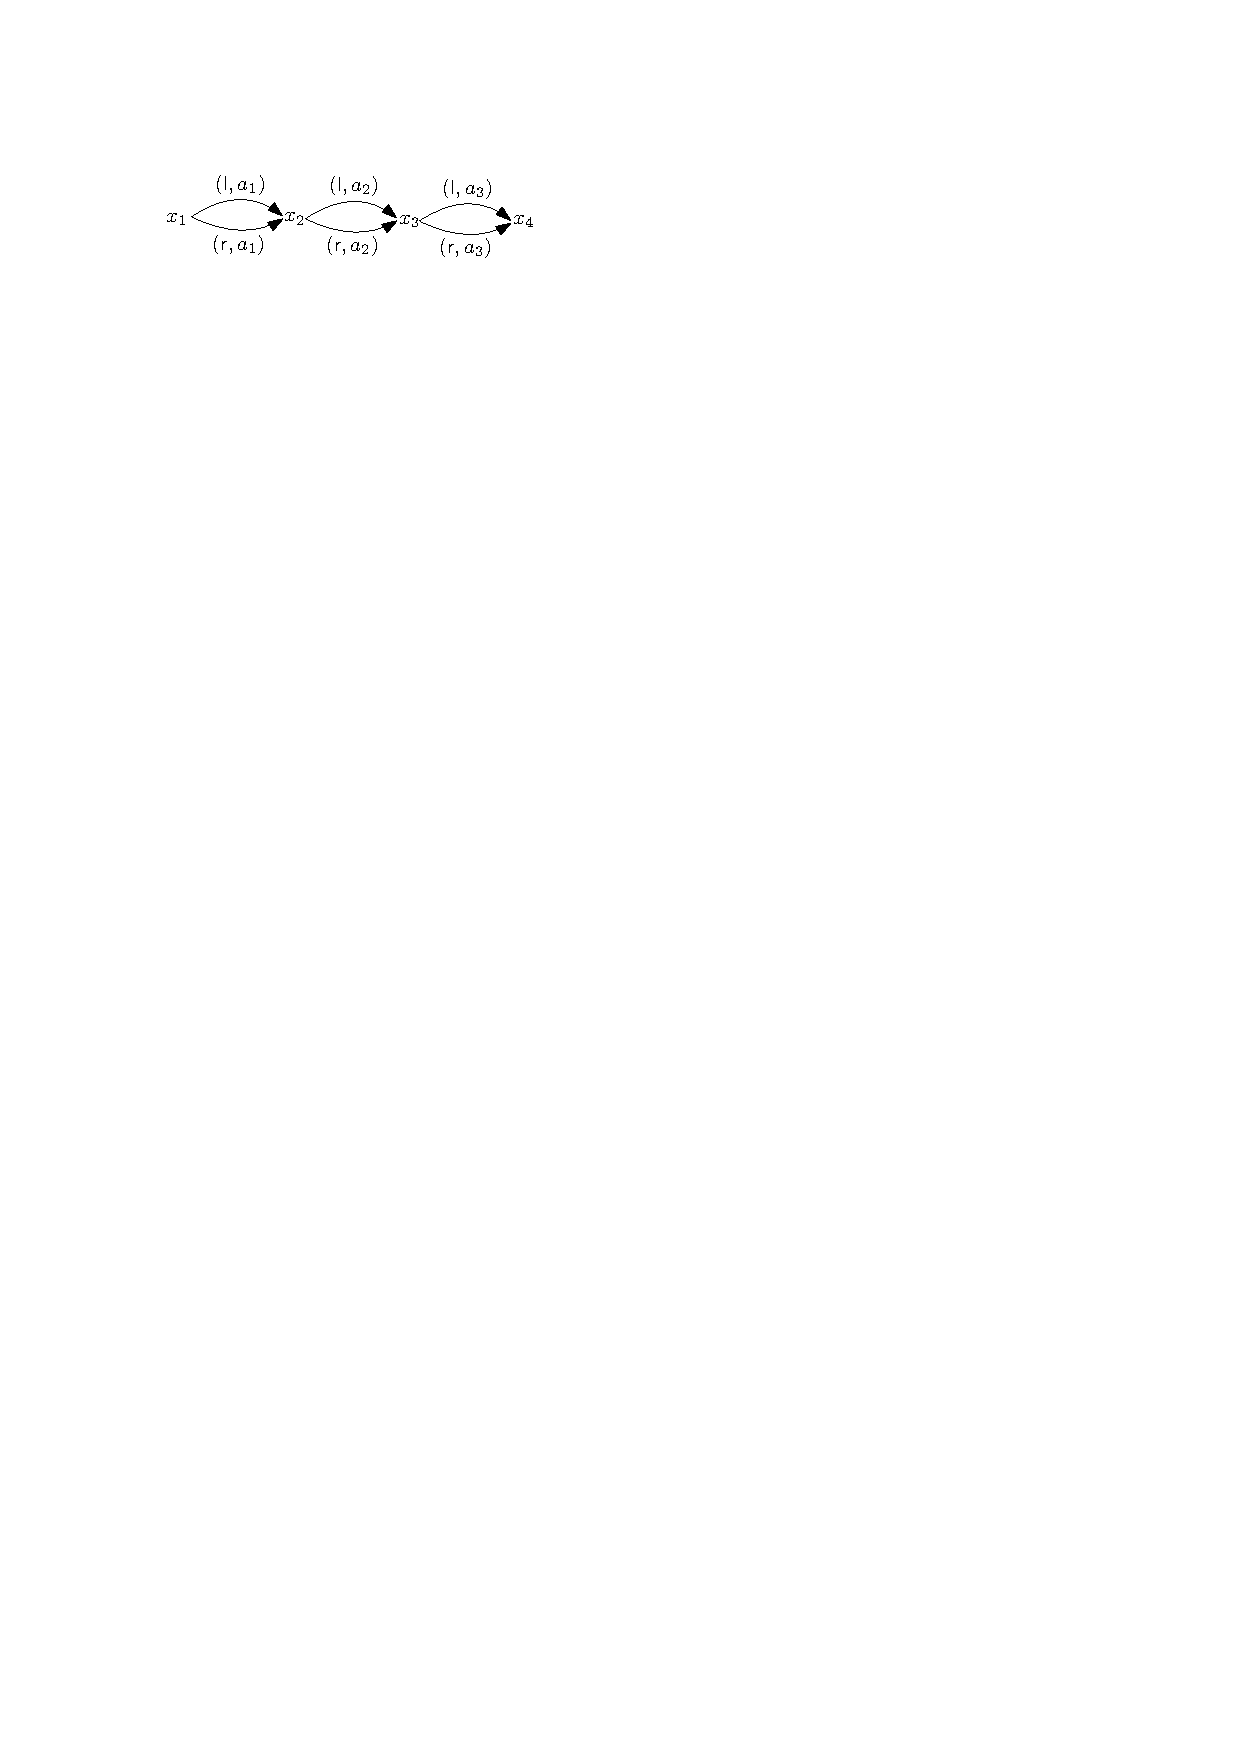
\includegraphics[scale=0.7]{dmdidx-example.pdf}
\end{center}
\caption{The diamond index  and the number of paths in $G_C$}\label{fig-dmdidx-exmp}
\end{figure}
\end{example}

In Section~\ref{sec:replaceallsl}--\ref{sec:replaceallre}, we will apply a refined analysis of the complexity of the decision procedures for proving Theorem~\ref{thm-main} and get the following results.

\begin{corollary}\label{cor-pspace}
The satisfiability problem is PSPACE-complete for the following fragments of $\strline[\replaceall]$:
\begin{itemize}
\item the single-letter case, plus the condition that the diamond indices of the dependency graphs are bounded by a constant $c$, 
%
\item the constant-string case, plus the condition that the $\rpleft$-lengths of the dependency graphs are bounded by a constant $c$, 

%
\item the regular-expression case, plus the condition that the $\rpleft$-lengths of the dependency graphs are at most $1$.
\end{itemize}
\end{corollary}

Corollary~\ref{cor-pspace} partially justifies our choice to present the decision procedures for the single-letter, constant-string, and regular-expression case separately. Intuitively, when the pattern parameters of $\replaceall$ terms become less restrictive, the decision procedures become more involved, and more constraints should be put on the dependency graphs in order to achieve the PSPACE upper bound. The PSPACE lower bound follows from the observation that the nonemptiness of the intersection of the regular expressions $e_1, \cdots, e_n$ over the alphabet $\{0,1\}$, which is a PSPACE-complete problem, can be reduced to the satisfiability of the formula $y = \replaceall((a b)^n, a, x) \wedge x \in (0+1)^\ast \wedge y \in e_1 \circ b  \circ \cdots \circ b \circ e_n$ (where $a, b \not \in \{0,1\}$), which belongs to all fragments in Corollary~\ref{cor-pspace}.\zhilin{Remark for the pspace lower bound, please check.}

%The proof of Theorem~\ref{thm-main} utilises a concept of dependency graphs defined below.



%Therefore,  in the following, without loss of generality, we assume that 
%in each $\strline[\replaceall]$ constraint $C=\varphi \wedge \psi$, the concatenation symbol $\concat$ does not occur in $\varphi$. 
 

